\chapter{Metastability and phononic CDW quench in TaTe2}

Strongly correlated condensed matter systems are materials with a very high complexity, making it difficult to predict and understand their properties.
To reduce this complexity Novoselov, Geim and co-workers proposed Graphene as a model system for more complex materials \cite{novoselov_electric_2004, novoselov_two-dimensional_2005, geim_rise_2007}.
Since then, researchers were extremely successful in finding new physical properties of Graphene itself while also extending and applying the knowledge to other materials.
Apart from the simplicity of these 2D materials, the idea of engineering properties by stacking multiple layers with different stacking orders or at twist angles offered the possibility of a vast playground for discovering and engineering new properties.
This resulted in the explosion of the field with the discovery of many new phenomena, from the observation of quatum Hall effect \cite{zhang_experimental_2005} to superconductivty in magic angle twisted bilayer graphene \cite{cao_unconventional_2018}.
Ultimately these developments lead the emergence other 2D material platforms.
One of these platforms of 2D materials are transition metal dichalcogenides (TMDCs) \cite{butler_progress_2013, chowdhury_progress_2020, liu_van_2016}.

These layered TMDs exhibit various phenomena xyz


One member of TMDC family is \ce{TaTe2} which, compared to its \ce{TaX2} based sister compounds \ce{TaS2} and \ce{TaSe2} and the isostructural polytypes of \ce{MTe2} like \ce{NbTe2} or \ce{VTe2}, it has so far received less attention from the community, but some reports characterizing the compound have come up in recent years, as well as the first ultrafast out-of-equilibrium studies.

Here talk more about the MTe and TaX properties (see RRR intro)

\ce{TaTe2}-crystals form in orthorombic (1T) structures, although in bulk crystals the 1T-phase is only a virtual phase and only exists in a distorted 1T' phase up to highest temperatures measured ($>$\qty{500}{\kelvin}).
The 1T phase has only been realized in epitaxilly grown mono and few-layer systems, which can form due to the absence or only weakly existing \ce{Te}-\ce{Te} interlayer coupling \cite{}. cite hwang , wang
In the real distorted 1T' phase, \ce{TaTe2} forms ribbon like structures and shows an overall (3 x 1) superstructure at the surface.
The structural distortion is governed by the local bonding, with \ce{Ta} atoms forming in trimers or fluctuating dimers, with each \ce{Ta}-atoms being surrounded by 8 \ce{Te}-atoms.
At \qty{170}{\kelvin} the material undergoes a structural phase transitions, where two \ce{Ta}-atoms further distort the structure, breaking dimers and instead form "butterfly" shaped heptameres in a (3 x 3) 1T"-phase \cite{feng_charge_2016, katayama_observation_2023}.
Simultaneously the stripe-like charge ordering at RT is modulated by the structural distortion and a hexagonal "star of david"-like charge order occurs below the phase transition.
This structural phase transition and the formation of the LT commensurate charge density wave (CDW), which has been observed both by gap formation (close to $E_F$) in ARPES \cite{lin_evidence_2022, mitsuishi_unveiling_2024} and the formation of a periodic lattice distortion (PLD) in STM and diffraction \cite{feng_charge_2016, siddiqui_ultrafast_2021, domrose_femtosecond_2024}.
The exact mechanism of how this phase transition occurs and what the interplay with the CDW is have still not been understood.

\begin{figure}
	\centering
	\begin{subfigure}[b]{0.3\textwidth}
		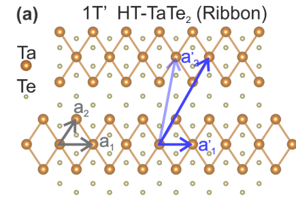
\includegraphics[width=\textwidth]{tate2/ht_structure.png}
	\end{subfigure}
	\hfill
	\begin{subfigure}[b]{0.3\textwidth}
		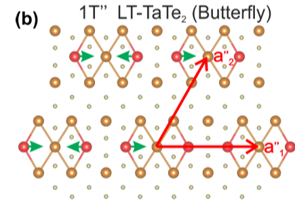
\includegraphics[width=\textwidth]{tate2/lt_structure.png}
	\end{subfigure}
	\hfill
	\begin{subfigure}[b]{0.3\textwidth}
		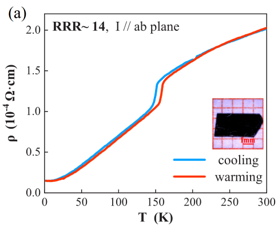
\includegraphics[width=\textwidth]{tate2/resistivity.png}
	\end{subfigure}
	\caption{(a) 1T' RT phase of \ce{TaTe2} forming ribbons. (b) 1T" LT phase of \ce{TaTe2}, \ce{Ta} atoms move together forming heptameres. (c) Resistivity of \ce{TaTe2} as a function of temperature with an overall reduction in resistivity while cooling. A phase transition occurs at \qty{170}{\kelvin}, which is accompanied by a further steplike reduction in resistivity.}
	\label{fig:tate_structure}
\end{figure}


The reason for the lack of understanding stems from the electronic reaction to the phase transition, especially in comparison to the \ce{TaX2} sister compounds.
Typically, entering a CDW phase by cooling the sample down from RT leads to an increase in resistivity due to the reduced density of states (DOS) in proximity to the Fermi level $E_F$.
Similarly the loss in DOS and with it the loss of electrons carrying magnetic moments should lead to a drop of the magnetic susceptibility while cooling through $T_s$.
Instead \ce{TaTe2}, which inhibits semi-metallic behavior at RT, shows a drop in resistivity and an increase in magnetic susceptibility, despite the observation of small gaps in the band structure \cite{sorgel_new_2006,hu_optical_2022,lin_evidence_2022}.
For this reason the compound has been branded a "strange" CDW material.

In this chapter of the thesis I give further insight into the driving mechanism of the CDW and the formation of the structural phase transition with the help of ultrafast pump-probe ARPES, and comparing our data to the recent ARPES and ultrafast publications on \ce{TaTe2}.
I will first introduce the band structure of \ce{TaTe2} and the Fermi surface topology, comparing the RT and LT phase, including the formation of CDW minigaps (first observed by \cite{lin_evidence_2022}).
After this I will give a description of the charge dynamics on a few picosecond timescale, including the delayed response of the CDW.
And then focus on the strong, band specific oscillations observed in the time domain and analyzing the different oscialltion modes with the help of Fourier analysis.
Last, I present a metastable electronic state persisting for $>\qty{200}{\pico\second}$ and discuss it's relevancy for the phase structural phase transition at equilibrium.

\section{Bandstructure and Fermiology}

The electronic structure of \ce{TaTe2} is characterized by local molecular bonding of the Ta-Ta dimers, with a strong orbital character.
Studying the band structure with ARPES reveals a complex set of bands at RT.
The valence states, which are governing the electronic properties of the compound consist of a mix of Ta 5d and Te 5p orbitals. \cite{mitsuishi_unveiling_2024}

The Fermi surface of \ce{TaTe2} shows a much stronger quasi-1D character when compared to other 2D materials, even the isostructural \ce{TaSe2} and \ce{TaS2}.
This character can be observed by 2-fold symmetric wavy contours around \qty{0.5}{\angstrom^{-1}}, which are located along the $\Gamma$-M$_1$ direction and forms an outer Fermi surface.
Within these contours, an inner second Fermi surface forming multiple pockets can be located (see Fig. \ref{fig:TaTe_FS}).

\begin{figure}[h!]
	\centering
	\begin{subfigure}[b]{0.5\textwidth}
		\includegraphics[width=\textwidth]{tate2/TaTe2_BZ_sketch_full.pdf}
		\caption{}
	\end{subfigure}
	\hfill
	\\
	\begin{subfigure}[b]{0.49\textwidth}
		\includegraphics[width=\textwidth]{tate2/TaTe2_FS_RT.pdf}
		\caption{}
	\end{subfigure}
	\hfill
	\begin{subfigure}[b]{0.49\textwidth}
		\includegraphics[width=\textwidth]{tate2/TaTe2_FS_LT.pdf}
		\caption{}
	\end{subfigure}
	\caption{(a) The measured Fermi surface of the LT phase is overlapped with the 1. BZ of the virtual monoclinic (1 x 1) 1T phase (black), extended BZs of the distorted HT (3 x 1) 1T' phase (orange) and extended BZs of the further distorted LT (3 x 3) 1 T'' phase (red). (b) RT Fermi surface overlapped with the HT and LT Brillouin zones. The relevant high symmetry points are marked. (c) Same Fermi surface as (b) but measured in the LT phase at \qty{77}{\kelvin}.}
	\label{fig:TaTe_FS}
\end{figure}

Comparing the RT and LT Fermi surface, only small changes can be observed.
The overall topology, consisting of the wavy outer contours and an inner FS sheet with multiple pockets is conserved.
A main difference lies in the slightly changed size of the pockets in the inner sheet, as some more pronounced features in the 2nd BZ of the LT FS.
The difference in size of the pockets stems from a slightly shifted chemical potential, when cooling through the phase transition, which has also been observed by N. Mitsuishi et. al. \cite{mitsuishi_unveiling_2024}.

Instead of the small changes in the Fermi surface topology, the effects of the phase transition become apparent when investigating the bandmaps.
Here, we compare a series of bandmaps taken parallel to the K$_2$-$\Gamma$-K$_2$ direction from the $\Gamma$-point to the edge of the 2nd BZ, for both room and low temperature.

\begin{figure}[t!]
	\centering
	\includegraphics[width=0.9\textwidth]{tate2/TaTe2_RT_cuts.pdf}
	\caption{Series of cuts parallel to K$_1$-$\Gamma$-K$_1$, from $\Gamma$ to the BZ border. The location of the cuts in respect to the BZ is indicated in the FS of Fig. \ref{fig:TaTe_FS}. All cuts have been taken at RT, using the Helium $\alpha1$ line of a Helium lamp.}
	\label{fig:TaTe_RT_cuts}
\end{figure}

The RT bandmaps show a manifold of bands, with multiple bands crossing the Fermi level in each cut.
These Fermi crossings clearly show the two different Fermi sheets, with the crossing at the edge of the cut determining the wavy contours of the outer quasi-1D Fermi surface sheet, and the crossing close to the center of the band structure forming the 2nd, inner Fermi sheet.
Cooling the compound through the phase transition results in a complex reordering of the bands.
The broader bands from the RT phase split in multiple individual ones, with additional backfolded bands appearing.
Looking at the FS crossing of the inner sheet, the aforementioned size difference of the Fermi pockets becomes clearer.
Comparing the cuts of the RT phase to the equivalent LT cuts, it is possible to identify a small shift in the chemical potential $\mu$, which has also been reported by \cite{mitsuishi_unveiling_2024}.
Another difference between the two phases is a band flattening close to $E_F$ at energies above \qty{-0.6}{\electronvolt}.

\begin{figure}[h]
	\centering
	\includegraphics[width=0.9\textwidth]{tate2/TaTe2_LT_cuts.pdf}
	\caption{Series of cuts parallel to K$_2$-$\Gamma$-K$_2$, from $\Gamma$ to the BZ border. The cuts are the equivalent band maps to the RT one in Fig. \ref{fig:TaTe_RT_cuts}. All cuts have been taken at LT $\simeq$\qty{77}{\kelvin}, using the Helium $\alpha1$ line of a Helium lamp.}
	\label{fig:TaTe_LT_cuts}
\end{figure}

This flattening of the bands might stem from the established charge order due to the CDW phase, typically resulting in the opening of gaps and backfolded bands from the PLD.
To further address the CDW and the gap formation we have to revisit the quasi-1D character of the FS.
A nesting of the FS occurs when different parts of the Fermi surface can be connected by a reciprocal lattice vector which can translate the different parts on top of each other.
This Fermi surface nesting (FSN) leads then to charge instabilities close to the FS and can play a dominant role in the formation of CDWs.
The wavy contours of the outer FS sheet (see Fig. \ref{fig:TaTe_FS}) fulfill the Fermi surface nesting (FSN) conditions.
Determining the distance between two points that are connected by this vector results in a length of approximately \qty{0.92}{\angstrom^{-1}}, which is comparable to the \qty{0.85}{\angstrom^{-1}} found by Y. Lin et al. \cite{lin_evidence_2022}.
A possible second FSN vector can be found for the inner FS sheet.
These bands show a stronger 1D character and the vector has a length of \qty{0.24}{\angstrom^{-1}}.
Both of these FSN vector lengths do not correspond to the periodicity of the PLD, which was found to be $simeq\qty{0.67}{\angstrom^{-1}}$.
The discrepancy between these vector lengths means that the FSN is not the sole driving force of the phase transition, underlining the complexity of the situation in \ce{TaTe2}.

As a result of the CDW formation minigaps can be observed across the Brillouin zone, most prominently close to the $\Gamma$-point \cite{lin_evidence_2022}.
Figure \ref{fig:TaTe_minigaps} shows a cut close to $\Gamma$, with a dashed box around the area in which the minigap formation occurs.
A zoom of this region better showcases these small gaps at the edge of the band map at around \qty{0.4}{\angstrom^{-1}}.
This band also connects to the wavy contours, which fulfill the FSN condition, further underlining the relevance for the CDW.

\begin{figure}[h!]
	\centering
	\includegraphics[width=0.7\textwidth]{tate2/TaTe2_CDW_minigaps.pdf}
	\caption{Left: Band map parallel to the K$_2$-$\Gamma$-K$_2$ direction close to the $\Gamma$-point. The dashed rectangle marks the region of which a zoom is provided. Right: Zoom of dashed rectangle region. The band map shows a faint signature of the observed minigaps \cite{lin_evidence_2022}.}
	\label{fig:TaTe_minigaps}
\end{figure}

\section{Ultrafast charge dynamics and CDW quench}

Investigating the evolution of the electronic band structure after pump excitation provides insight into the relaxation dynamics, not only of an isolated electronic states, but also the collective response of the material out of equilibrium.
Performing pump-probe experiments at RT and LN temperature allows us to reveal differences between the two different structural phases.
The excitation is created by a \qty{1.55}{\electronvolt} ultrashort laser pulse.
Here, I will first analyze measurements that have been performed in the low temperature phase at \qty{77}{\kelvin} and then switch to RT data to point out the differences due to the phase transition.

The LT cuts, presented in this section, have been measured parallel to K$_2$-$\Gamma$-K$_2$ direction at three different points in the LT FBZ ($\Gamma$, M$_1$ and in proximity of $\Gamma$ See Fig. ref).
Focusing on the cut close to $\Gamma$ it is possible to make out a complex band dynamics, depending on the region in the band structure.
Figure \ref{fig:TaTe_bandmap_dyn_betw} shows this band map \qty{50}{\femto\second} after excitation.
Additionally, difference maps for three different time steps (\qtylist{50; 500; 4000}{\femto\second}) are plotted to better display the pump-induced changes.

At \qty{50}{\femto\second} a fast depopulation of occupied bands can be observed, with the difference band contours following the band structure at equilibrium.
Similarly a fast population of the unoccupied states occurs.
This is followed by the decay of the excitation, but at \qty{500}{\femto\second} a sudden increase in spectral weight occurs in the occupied states.
This atypical behavior can be explained by a quench of the charge order, and will be discussed in greater detail when analyzing specific delay traces at the end of this section.
At a time delay of \qty{4}{\pico\second} most of the population in the excited states has decayed, but a rest population is still observed.
Additionally the band structure is significantly altered compared to the equilibrium state.

\begin{figure}[t!]
	\centering
	\includegraphics[width=\textwidth]{tate2/bandmap_dyn_markers_betw.pdf}
	\caption{Left: Band map close to $\Gamma$ oriented along K$_2$-$\Gamma$-K$_2$ direction at a time delay of \qty{50}{\femto\second} after pump excitation. The other plots show difference maps at different time delays (\qtylist{50;500;4000}{\femto\second}). Rectangles show the regions for which dedicated delay traces are displayed in \ref{fig:TaTe_dyn_betw}. The difference map show characteristic features for each time steps. At \qty{50}{\femto\second} fast de-/population due to the pump excitation occurs. After \qty{500}{\femto\second} a population of a region below $E_F$ appears, corresponding to the closure of the CDW gap. After \qty{4}{\pico\second} the difference map shows regions where a change of the band structure and population above $E_F$ persists. Measurement was done at \qty{77}{\kelvin}.}
	\label{fig:TaTe_bandmap_dyn_betw}
\end{figure}

Some exemplary traces have been selected for a more detailed insight into the relaxation dynamics.
These traces are marked with squares in the band maps, black squares for the unoccupied band structure, white for the occupied region and green for the region with a significant spectral weight after \qty{4}{\pico\second}.
Traces for the unoccupied region (black squares, see Fig. \ref{fig:TaTe_dyn_betw} (a)-(c)) shows a sharp population within the duration of the pump pulse.
The ultrafast population is followed by a fast decay which becomes increasingly longer when approaching $E_F$.
In each trace, the population has decayed within \qty{4}{\pico\second}.
Similarly the depopulation of the occupied state in Fig. \ref{fig:TaTe_dyn_betw} (d) is created within the pump pulse duration and recovers on the same time scale.

Unexpected dynamics occur when looking at the region that shows a increase in population below $E_F$.
Typically a pump light pulse excites the system which transfers energy to electrons and drives a transition to a higher unoccupied state, therefore reducing the occupancy below $E_F$.
Instead \ce{TaTe2} shows small gaps resulting from the CDW, which leads in the LT phase to a loss of density of states (DOS), when compared to the RT phase.
If this charge order is broken, the gap closes and in a simple case, excluding other band modifications, the DOS of the RT phase is re-established.
This behavior is observed in Fig. \ref{fig:TaTe_dyn_betw} (e), which coincides with the region of CDW gaps reported by \cite{lin_evidence_2022}.
Strikingly, the breaking of the CDW order does not occur at $t_0$.
Fitting a single exponential decay model retrieves a time zero of $t_0=\qty{388}{\femto\second}$, introducing a significant delay of approximately \qty{320}{\femto\second} when compared to the time zero of all other curves.

This delayed response becomes very apparent, when the delay trace is overlapped with the dynamics of the fast de- or population (see Fig. \ref{fig:TaTe_CDW_comp}).
Many ultrafast studies have looked at the dynamics of the CDW and while the timescales typically differ, depending on the mechanism, a common observation is that the quench of the charge order starts together with the arrival of the pump pulse. \cite{} rossnagel etc.
In contrast, here a quench on the timescale of few hundred \unit{\femto\second} is observed, which would traditionally be associated with a Peierls type CDW, but the onset of the quench is delayed with respect to time zero $t_0$.
The delayed response rules out a solely electronic character and instead established the structural component as the dominant contribution for the CDW order in \ce{TaTe2}.
In other words, instead of the electromagnetic field of the pump pulse directly disrupting the charge order e.g. via buildup of free charges and subsequent screening, the more likely scenario is an coherent response of the lattice to the intense light illumination, resulting in an excitation of phonon modes on ultrafast time scales, which couple to the charge order via the strong electron-phonon coupling of the system.

\begin{figure}[t]
	\centering
	\begin{subfigure}[b]{0.33\textwidth}
		\includegraphics[width=\textwidth]{tate2/Unocc_dyn_1_fit_betw.pdf}
		\caption{}
	\end{subfigure}
	\hfill
	\begin{subfigure}[b]{0.33\textwidth}
		\includegraphics[width=\textwidth]{tate2/Unocc_dyn_2_fit_betw.pdf}
		\caption{}
	\end{subfigure}
	\hfill
	\begin{subfigure}[b]{0.33\textwidth}
		\includegraphics[width=\textwidth]{tate2/Unocc_dyn_3_fit_betw.pdf}
		\caption{}
	\end{subfigure}
	\\
	\begin{subfigure}[b]{0.33\textwidth}
		\includegraphics[width=\textwidth]{tate2/Occ_dyn_fit_betw.pdf}
		\caption{}
	\end{subfigure}
	\hfill
	\begin{subfigure}[b]{0.33\textwidth}
		\includegraphics[width=\textwidth]{tate2/CDW_quench_fit_betw.pdf}
		\caption{}
	\end{subfigure}
	\hfill
	\begin{subfigure}[b]{0.33\textwidth}
		\includegraphics[width=\textwidth]{tate2/Meta_dyn_fit_betw.pdf}
		\caption{}
	\end{subfigure}
	\caption{Delay traces of the regions marked in Fig. \ref{fig:TaTe_bandmap_dyn_betw} with the corresponding fit function of a single exponential decay model and resulting time constants $t_0$ and $\tau$. (a)-(c) Dynamics of unoccupied regions (black markers in Fig. \ref{fig:TaTe_bandmap_dyn_betw}) show fast population within pump pulse, followed with increasing relaxation time closer to $E_F$. (d)-(e) Dynamics of unoccupied regions (white markers in Fig. \ref{fig:TaTe_bandmap_dyn_betw}). (d) Fast depopulation within pump excitation. (e) Delayed response compared to $t_0$ and increased spectral weight. (f) Dynamics of region slightly above $E_F$ (green marker in Fig. \ref{fig:TaTe_bandmap_dyn_betw}) shows a instantaneous population within pump pulse, and persisting occupation beyond \qty{4}{\pico\second}.}
	\label{fig:TaTe_dyn_betw}
\end{figure}

The unresponsiveness of the CDW to the direct light illumination shows as well when looking at a region at the edge of the CDW gap, also containing the part of the gapped band.
The corresponding dynamics, overlapped with the dynamics of the direct de-/population are shown in Fig. \ref{fig:TaTe_CDW_comp}.
In the trace an inital dip at $t_0$ can be seen, originating from the depopulation dynamics of the occupied band.
But after \qty{300}{\femto\second}, this depopulation is downed out by the closing of the CDW gap.
It is quite remarkable that in adjacent energy-momentum coordinates an instantaneous reaction to the occupied band dynamics is observed while the CDW only shows a delayed response, which speaks for the strong structural character of the established order.
A relaxation time of $\tau_{CDW}=\qty{500}{\femto\second}$ can be extracted by fitting a single exponential decay model, corresponding to the time duration to reestablish the charge order.

\begin{figure}[t!]
	\centering
	\begin{subfigure}[b]{0.33\textwidth}
		\includegraphics[width=\textwidth]{tate2/CDW_quench_multitrace_betw.pdf}
		\caption{}
	\end{subfigure}
	\begin{subfigure}[b]{0.33\textwidth}
		\includegraphics[width=\textwidth]{tate2/CDW_2_dyn_fit.pdf}
		\caption{}
	\end{subfigure}
	\caption{Left: Delay trace showing the dynamics of the CDW quench, overlapped with delay traces showing the direct de-/population of the occupied/unoccupied states, visualizing the delayed response of the CDW to the light excitation. Right: Dynamics of CDW quench combined with a fit of a single exponential decay model, resulting in a decay time of $\tau_{CDW}=\qty{460}{\femto\second}$ and an onset of the dynamic at $t=\qty{420}{\femto\second}$.}
	\label{fig:TaTe_CDW_comp}
\end{figure}

Coming back to the residual spectral weight visible in the difference map at \qty{4}{\pico\second} in Fig. \ref{fig:TaTe_bandmap_dyn_betw}, the corresponding delay trace of the green square (see Fig. \ref{fig:TaTe_dyn_betw}) shows the same fast population within the pump pulse duration, with an initial decay, but the population does not return to the initial state.
Instead a sharp feature is visible above $E_F$.
A more detailed analysis of this feature, including measurements on longer time scales, will be done in section \ref{sec:meta}.
Also a common feature in the delay traces are strong coherent oscillation of the intensity.
A detailed analysis of these oscillations will also be tackled in the next sectionm\ref{sec:phonon_osc}.

This series of dynamics is not only visible in proximity to $\Gamma$ but can also be observed directly at $\Gamma$, as well as at the edge of the FBZ at M$_1$.
Figure \ref{fig:TaTe_bandmap_dyn_bzb} shows the excited bandmap at $t_0$, followed by difference maps at specific time delays.
In both, the same instantaneous de-/population of the occupied/unoccupied bands is visible, as well as a quench of a CDW gap that also shows a delayed response of multiple hundreds of \unit{\femto\second} (see Fig. \ref{fig:TaTe_bandmap_dyn_bzb} (c)-(d)).
The only difference in the dynamics is an absence of residual spectral weight at M$_1$, but this measurement has been performed at a lower pump fluence, which is the reason for the absence.

\begin{figure}[t!]
	\centering
	\includegraphics[width=\textwidth]{tate2/bandmap_dyn_markers_betw_rt.pdf}
	\caption{Left: Band map close to $\Gamma$ oriented along K$_2$-$\Gamma$-K$_2$ direction \qty{50}{\femto\second} after pulse excitation. The other plots show difference maps at different time delays (\qtylist{50;400;3000}{\femto\second}). Rectangles show the regions for which dedicated delay traces are displayed in \ref{fig:TaTe_dyn_betw_RT}. The difference map shows the ultrafast de-/population after pump excitation, followed by a decay and a small diffuse residual spectral weight after \qty{3}{\pico\second}. No changes to the band structure apart from de-/population dynamics can be observed.}
	\label{fig:TaTe_bandmap_dyn_betw_rt}
\end{figure}

Comparing the dynamics of the LT phase to the RT phase, reveals significant differences for the same cut of band structure (see Fig. \ref{fig:TaTe_bandmap_dyn_betw_rt} cut close to $\Gamma$).
First a direct population of the occupied states can be observed within the pump pulse duration.
But, unlike the LT case, the population seems to be disproportionately located in the region just above $E_F$, whereas the unoccupied states at higher energies appear to be less populated.
While the LT phase was additionally characterized by strong changes to the band structure after the first few hundred \unit{\femto\second}, no changes occur in the RT phase.
Instead, the population of the unoccupied bands, as well as the depopulation of the occupied parts simply decays.
After \qty{3}{\pico\second} some spectral weight still remains close to $E_F$, but no discrete spectral feature can be observed.
The full time dynamic for selected regions can be seen in Fig. \ref{fig:TaTe_dyn_betw_rt}.
Those traces show similar relaxation times as the LT ones.
Similar observations can be made for the other cuts at RT.

\begin{figure}[b!]
	\centering
	\begin{subfigure}[b]{0.24\textwidth}
		\includegraphics[width=\textwidth]{tate2/Unocc_dyn_1_fit_betw_rt.pdf}
		\caption{}
	\end{subfigure}
	\begin{subfigure}[b]{0.24\textwidth}
		\includegraphics[width=\textwidth]{tate2/Unocc_dyn_2_fit_betw_rt.pdf}
		\caption{}
	\end{subfigure}
	\begin{subfigure}[b]{0.24\textwidth}
		\includegraphics[width=\textwidth]{tate2/Unocc_dyn_3_fit_betw_rt.pdf}
		\caption{}
	\end{subfigure}
	\begin{subfigure}[b]{0.24\textwidth}
		\includegraphics[width=\textwidth]{tate2/Occ_dyn_fit_betw_rt.pdf}
		\caption{}
	\end{subfigure}
	\caption{
		Delay traces of the regions marked in Fig. \ref{fig:TaTe_bandmap_dyn_betw_rt} with the corresponding fit function of a single exponential decay model and resulting time constants $t_0$ and $\tau$. (a)-(c) Dynamics of unoccupied regions (black markers in Fig. \ref{fig:TaTe_bandmap_dyn_betw_rt}) show fast population within pump pulse, followed with increasing relaxation time closer to $E_F$. (d) Dynamic of unoccupied regions (white markers in Fig. \ref{fig:TaTe_bandmap_dyn_betw_rt}) shows fast depopulation within pump excitation and small residual spectral weight after \qty{3}{\pico\second}.}
	\label{fig:TaTe_dyn_betw_rt}
\end{figure}

With these results in mind, two key differences are apparent from the RT data.
First is the lack of a spectral feature appearing around \qty{500}{\femto\second}, as well as no band reordering.
This is expected, since there are no CDWs or any resulting CDW gaps in the RT phase.
Second, while there is still some residual spectral weight left after \qty{3}{\pico\second}, there are no sharp features visible.
Instead the spectral weight seems to have a diffuse distribution around the occupied bands.
Additionally, there is no band reordering associated with this residual spectral weight.



\begin{figure}[h!]
	\centering
	\begin{subfigure}[b]{\textwidth}
		\includegraphics[width=\textwidth]{tate2/bandmap_dyn_markers_gamma.pdf}
		\caption{}
	\end{subfigure}
	\\
	\centering
	\begin{subfigure}[b]{\textwidth}
		\includegraphics[width=\textwidth]{tate2/bandmap_dyn_markers_bzb.pdf}
		\caption{}
	\end{subfigure}
	\\
	\begin{subfigure}[b]{0.33\textwidth}
		\includegraphics[width=\textwidth]{tate2/CDW_quench_multitrace_gamma.pdf}
		\caption{}
	\end{subfigure}
	\begin{subfigure}[b]{0.33\textwidth}
		\includegraphics[width=\textwidth]{tate2/CDW_quench_multitrace_bzb.pdf}
		\caption{}
	\end{subfigure}
	\caption{Figure similar to Fig. \ref{fig:TaTe_bandmap_dyn_betw} for different cuts. (a) Cut through $\Gamma$. (b) Cut through M$_1$. Both cuts are along the K$_2$-$\Gamma$-K$_2$ direction. (c) \& (d) show trace of the CDW quench plotted together with the direct excitation of the unoccupied states.}
	\label{fig:TaTe_bandmap_dyn_bzb}
\end{figure}

\section{Energy and momentum resolved electron-phonon coupling}
\label{sec:phonon_osc}

The previous section was dedicated to the dynamics both at LT and RT.
Those dynamics already revealed strong oscillations in the intensity of each trace, which will be the subject of this section.

Coherent oscillations in delay traces of a trARPES measurement typically are a sign of interaction with phonons.
Since ARPES only measures the single particle wavefunction of photoemitted electrons, it is not possible to directly observe quasiparticles like phonons.
But the information of phonons is still imprinted into the measured photoelectrons due to the electron-phonon coupling.
If this electron-phonon coupling becomes sufficiently large it is possible to observe oscillations is the time traces of a trARPES experiment.
Tellurides, and especially \ce{TaTe2} seem to carry an exceptionally high electron-phonon coupling.
Due to this, it is not only possible to observe oscillations in a large, integrated region of the band structure, but rather for each momentum and energy coordinate individually.
With this it is possible to perform a band mapping of the electron-phonon coupling constant in a large energy-momentum region.
Additionally, by carrying out a fourier analysis of the delay trace we can extract the frequency of the oscillation and assign it to known vibrational modes.

For this procedure a small binning of four pixel in both the momentum and energy coordinate is applied to the raw data to slightly increase the signal to noise ration and reduce the amount of pixels for which the calculations have to run while slightly reducing the fidelity of the bandmaps.
After this, a single exponential decay model is fit to each $E(k)$-coordinate to account for the population decay.
The exponential decay is then subtracted from the raw data trace, only leaving a residual behind containing the oscillating component.
A fast Fourier transform function is then applied to the residual trace, revealing the frequency of the oscillatory components.
This transforms the original 3D data cube from $I(E,k,t)$ to $I(E,k,f)$, with frequency $f$ being the Fourier transformed of the the time axis.
Fig. \ref{fig:TaTe_fit_procedure} shows the steps from a delay trace to the FFT trace that can be associated with a particular phonon mode.

\begin{figure}[t!]
	\centering
	\includegraphics[width=\textwidth]{tate2/tate_fit_procedure.pdf}
	\caption{Left: Band map close to $\Gamma$ oriented along K$_2$-$\Gamma$-K$_2$ direction \qty{50}{\femto\second} after pulse excitation. The other plots show difference maps at different time delays (\qtylist{50;400;3000}{\femto\second}). Rectangles show the regions for which dedicated delay traces are displayed in \ref{fig:TaTe_dyn_betw_RT}. The difference map shows the ultrafast de-/population after pump excitation, followed by a decay and a small diffuse residual spectral weight after \qty{3}{\pico\second}. No changes to the band structure apart from de-/population dynamics can be observed.}
	\label{fig:TaTe_fit_procedure}
\end{figure}

Performing this analysis for a cut close to $\Gamma$ reveals 3 distinct vibrational modes in the LT phase (see Fig. \ref{fig:TaTe_FFT_betw} (c)) at \qtylist{0.4; 1.45; 2.3}{\tera\hertz}.
Two modes (\qtylist{1.45; 2.3}{\tera\hertz}) are well known phonon modes which have been oberserved with Raman spectroscopy and ultrafast transient reflectivity \cite{luo, hu_optical_2022}, while the \qty{0.4}{\tera\hertz} on the other hand has not been observed.
The resulting band maps for these three frequencies are shown in Fig. \ref{fig:TaTe_FFT_betw} (b) with the corresponding band structure \qty{50}{\femto\second} after pump excitation.
From these band maps it becomes clear that the individual phonon modes couple to different bands in the band structure.
Most strikingly, the features coupling to the \qty{0.4}{\tera\hertz} mode, are the bands that showed the CDW gap closing in the previous section.

\begin{figure}[h!]
	\centering
	\begin{subfigure}[b]{0.24\textwidth}
		\includegraphics[width=\textwidth]{tate2/tate_FFT_ref_betw.pdf}
		\caption{}
	\end{subfigure}
	\begin{subfigure}[b]{0.72\textwidth}
		\includegraphics[width=\textwidth]{tate2/tate_FFT_betw.pdf}
		\caption{}
	\end{subfigure}
	\\
	\begin{subfigure}[b]{0.33\textwidth}
		\includegraphics[width=\textwidth]{tate2/tate_FFT_summed.pdf}
		\caption{}
	\end{subfigure}
	\caption{Figure similar to Fig. \ref{fig:TaTe_bandmap_dyn_betw} for different cuts. (a) Cut through $\Gamma$. (b) Cut through M$_1$. Both cuts are along the K$_2$-$\Gamma$-K$_2$ direction. (c) \& (d) show trace of the CDW quench plotted together with the direct excitation of the unoccupied states.}
	\label{fig:TaTe_FFT_betw}
\end{figure}

\begin{figure}[bh!]
	\centering
	\begin{subfigure}[b]{\textwidth}
		\includegraphics[width=\textwidth]{tate2/Osc_time_traces_betw.pdf}
		\caption{}
	\end{subfigure}
	\\
	\begin{subfigure}[b]{\textwidth}
		\includegraphics[width=\textwidth]{tate2/Osc_freq_traces_betw.pdf}
		\caption{}
	\end{subfigure}
	\caption{Figure similar to Fig. \ref{fig:TaTe_bandmap_dyn_betw} for different cuts. (a) Cut through $\Gamma$. (b) Cut through M$_1$. Both cuts are along the K$_2$-$\Gamma$-K$_2$ direction. (c) \& (d) show trace of the CDW quench plotted together with the direct excitation of the unoccupied states.}
	\label{fig:TaTe_FFT_traces_betw}
\end{figure}

In Fig. \ref{fig:TaTe_FFT_traces_betw} some exemplary time traces are shown in (a) with their corresponding FFT trace in (b).
These traces help visualizing the difference in the modes and give further insight into their respective nature.
While the \qtylist{1.45; 2.3}{\tera\hertz} phonon modes oscillate around the exponential decay, it appears as if the \qty{0.4}{\tera\hertz} mode strongly modulates the intensity in the trace, almost resulting in a re-population after the decay has already set in.
Additionally, oscillations due to the electron-phonon coupling seem to set in right after the excitation with the IR pump pulse.
This observation agrees as well with the fact, that the CDW is not disrupted immediately by the light pulse, but through the interaction with the phonons, with the the CDW gap being quenched after \qty{350}{\femto\second}.
Similar observations can be made for the two other cuts at $\Gamma$ and M$_1$, that have been analyzed before in terms of their dynamics.
Both cuts show the three phonon modes listed above and show them couple to different bands in band structure.

One of the big questions in \ce{TaTe2} is about the nature of the CDW.
In the previous section I presented our results on strong structural character of the CDW, which became apparent through the delayed response to light excitation.
As a second part I want to address the question of an amplitude mode.
The main characteristic of a possible amplitude mode is that the mode vanishes after crossing from the CDW phase into the HT phase.
For this reason it is again necessary to look at the RT data and see how the oscillations change.

\begin{figure}[b!]
	\centering
	\begin{subfigure}[b]{0.33\textwidth}
		\includegraphics[width=\textwidth]{tate2/tate_FFT_ref_betw_rt.pdf}
		\caption{}
	\end{subfigure}
	\begin{subfigure}[b]{0.66\textwidth}
		\includegraphics[width=\textwidth]{tate2/tate_FFT_betw_rt.pdf}
		\caption{}
	\end{subfigure}
	\\
	\begin{subfigure}[b]{0.33\textwidth}
		\includegraphics[width=\textwidth]{tate2/tate_FFT_summed_rt.pdf}
		\caption{}
	\end{subfigure}
	\caption{Figure similar to Fig. \ref{fig:TaTe_bandmap_dyn_betw} for different cuts. (a) Cut through $\Gamma$. (b) Cut through M$_1$. Both cuts are along the K$_2$-$\Gamma$-K$_2$ direction. (c) \& (d) show trace of the CDW quench plotted together with the direct excitation of the unoccupied states.}
	\label{fig:TaTe_FFT_betw_rt}
\end{figure}

The first thing that becomes immediately apparent in RT data is the lack of the \qty{0.4}{\tera\hertz} mode (see Fig. \ref{fig:TaTe_FFT_betw_rt} (c)).
This absence is absence is a strong indicator that the mode might be an amplitude mode.
Other indicators are also present in the LT data, such as the \qty{0.4}{\tera\hertz} mode directly coupling to the region of CDW gaps, or the oscillations of the mode having the strongest effect on the observed intensity.
Apart from the changes to the potential Amplitude mode, additional changes to the two other modes are visible.
First, both modes experience a slight red shift compared to the LT data and seem to have broadened.
Second, the bands to which the \qty{1.35}{\tera\hertz} mode couples seems to have changed, while the \qty{2.2}{\tera\hertz} mode stayed the same (see Fig. \ref{fig:TaTe_FFT_betw_rt} (b)).
The \qty{1.35}{\tera\hertz} mode now incorporates a broader region in the band structure at the edge of the band map, as well as the band in the center, which coupled to the \qty{0.4}{\tera\hertz} mode at LT.

With these results in mind it is possible to provide further insight into the structural phase transition and the CDW formation.
Two phonon modes have been observed at LT, which persist up to RT.
Both of these modes have been previously observed by transient reflectivity and raman spectroscopy \cite{luo, hu_optical_2022}, although the \qty{1.45}{\tera\hertz} mode only appeared in the LT data of \cite{hu_optical_2022}.
I attribute the absence of this mode in the HT phase to the probe energy used in the transient reflectivity data.
The \qty{2.3}{\tera\hertz} is basically not effected by the phase transition, apart from a slight red shift which has also been reported by \cite{luo, hu_optical_2022}.
More importantly the band resolved electron-phonon coupling is also unchanged, therefore the \qty{2.3}{\tera\hertz} mode likely does not play a major role in the phase transition.
While the \qty{1.45}{\tera\hertz} also appears in both LT and HT phase, the band specific electron-phonon coupling changes quite significantly, especially in the center of the of BZ close to $\Gamma$ and in the location of the minigap formation.
In these regions the \qty{0.4}{\tera\hertz} mode appears at LT, coupling to the bands that are affected by the CDW gap formation.
A possible explanation for these observations could be the strong orbital character of the bands, and the different Ta d-orbitals which mainly make up the band structure close to $E_F$ \cite{mitsuishi_unveiling_2024}.
The orbital which is most affected by the structural phase transition is the $d_{xy}$ orbital, it is likely that the changed overlap due to the heptamere formation affects the electron-phonon coupling due to the localized bonding character of the material in general.
This would then allow for the CDW order to establish itself, mediated by the \qty{0.4}{\tera\hertz} phonon.

\section{Metastability}
\label{sec:meta}

Lastly I want to focus on the residual spectral weight, that was shown in the LT phase dynamics see \ref{fig:TaTe_bandmap_dyn_betw}.
Recently two groups have reported on a metastable state persisting into the \unit{\nano\second} regime, observed in pump probe electron diffraction measurements \cite{siddiqui_ultrafast_2021, domrose_femtosecond_2024}.
These results only provide insight on the structural dynamics of the material.
But especially for compounds with such strong electron-phonon coupling it is imperative to also understand the electronic side of the out of equilibrium dynamics in order to disentangle the multiple different reordering and relaxation processes.
In the previous sections I introduced the ultrafast electronic dynamics.
Here, I will concentrate on the possible long term modifications of the electronic band structure and the different time scales leading up to the metastable state.
For this measurements of the valence states at longer time scales have been performed, both at LT and RT, as well as pump probe measurements on the Te 4d core states.

\begin{figure}[t!]
	\centering
	\begin{subfigure}[b]{0.25\textwidth}
		\includegraphics[width=\textwidth]{images/tate2/meta_bandmap_marker}
		\caption{}
	\end{subfigure}
	\\
	\begin{subfigure}[b]{\textwidth}
		\includegraphics[width=\textwidth]{images/tate2/tate_lt_meta_steps}
		\caption{}
	\end{subfigure}
	\caption{(a) Bandmap of a cut close to $\Gamma$ along the K$_2$-$\Gamma$-K$_2$ direction similar to Fig. \ref{fig:TaTe_bandmap_dyn_betw} taken at $t_0$. Black markers show regions of the time traces shown in Fig. \ref{fig:metastableedge} (c)-(f). Region between two dashed lines corresponds to (a), region above higher dashed line to (b). (b) Difference maps showing the relative changes compared to before $t_0$ at selected time delays from $t_0$ to \qty{200}{\pico\second} after excitation. Measurement has been performed in the LT phase at approximately \qty{77}{\kelvin}.}
	\label{fig:tateltmetasteps}
\end{figure}

I will first focus on the dynamics of the band structure as a whole by looking at difference maps of a momentum cut close to BZ center.
The cut was taken in the LT phase at $\approx$\qty{77}{\kelvin} in the  K$_2$-$\Gamma$-K$_2$ direction, similar to Fig. \ref{fig:TaTe_bandmap_dyn_betw}.
In this measurement the range of delay steps was increased, measuring with a relatively fine step size of \qty{250}{\femto\second} from before $t_0$ to \qty{5}{\pico\second}, followed by progressively increased step sizes up to \qty{200}{\pico\second} after pulse excitation.
The corresponding band map \qty{250}{\femto\second} after pulse excitation is shown in \ref{fig:tateltmetasteps} (a), together with the difference maps at selected time delays in Fig. \ref{fig:tateltmetasteps} (b).
In the first four difference maps between \qtyrange{250}{2000}{\femto\second} the same dynamics, which have been discussed in the previous section can be observed.
First an immediate de- \& population of the respective states occurs, which is followed by a delayed response of the charge order and a full quench of the CDW gaps $\approx$\qty{500}{\femto\second} after laser excitation.
The charger order recovers within \qty{1.5}{\pico\second} after the phonon mediated quench occurred.
During this recovery a reordering of the band structure sets in.
This transient reordering stabilizes after \qty{5}{\pico\second} and settles into band structure distinctly different from the equilibrium structure.
The new electronic structure is stable beyond \qty{200}{\pico\second} after excitation and fully recovers on \unit{\milli\second} timescales.

\begin{figure}[t!]
	\centering
	\begin{subfigure}[b]{0.33\textwidth}
		\includegraphics[width=\textwidth]{images/tate2/metastable_edge}
		\caption{}
	\end{subfigure}
	\begin{subfigure}[b]{0.33\textwidth}
		\includegraphics[width=\textwidth]{images/tate2/metastable_high}
		\caption{}
	\end{subfigure}
	\begin{subfigure}[b]{0.33\textwidth}
		\includegraphics[width=\textwidth]{images/tate2/metastable_occ}
		\caption{}
	\end{subfigure}
	\\
	\begin{subfigure}[b]{0.33\textwidth}
		\includegraphics[width=\textwidth]{images/tate2/metastable_state_ef}
		\caption{}
	\end{subfigure}
	\begin{subfigure}[b]{0.33\textwidth}
		\includegraphics[width=\textwidth]{images/tate2/metastable_left}
		\caption{}
	\end{subfigure}
	\begin{subfigure}[b]{0.33\textwidth}
		\includegraphics[width=\textwidth]{images/tate2/metastable_cdw}
		\caption{}
	\end{subfigure}
	\caption{Delay traces from \qtyrange{-1}{200}{\pico\second} for different regions close to $\Gamma$ as marked in Fig. \ref{fig:tateltmetasteps} (a) Inset shows a smaller time window (\qtyrange{-1}{10}{\pico\second}) with finer step size. Vertical dashed lines in the inset show the relaxation of the CDW and the coinciding band reordering at \qty{2}{\pico\second}. (a) Region close to the Fermi level, between the 2 dashed lines. (b) Region of unoccupied states at higher energies beyond (a). (c)-(f) Traces for regions marked with black squares. (c) Metastable depopulation of occupied state. (d) Metastable population of spectral feature above $E_F$, shows a delayed formation. (e) Fast depopulation of an occupied state, followed by a delayed reaction due to the band reordering. (f) Ultrafast depopulation of unoccupied state with CDW quench and subsequent band reordering. All traces taken at approximately \qty{77}{\kelvin}.}
	\label{fig:metastableedge}
\end{figure}

Following the time traces for selected features in the band structure provides a more detailed insight into the sequence of processes.
The selected traces are shown in Fig. \ref{fig:metastableedge}, with the corresponding regions of (c)-(f) marked by squares in Fig. \ref{fig:tateltmetasteps}.
Fig. \ref{fig:tateltmetasteps} (a) \& (b) correspond to the full range of momentum and for an energy $E_{kin}=E_F-E$ from \qtyrange{0}{0.15}{\electronvolt} or \qtyrange{0.15}{1.5}{\electronvolt} respectively (marked by the black dotted lines in Fig \ref{fig:tateltmetasteps} (a)).
The traces of (a) \& (b) illustrate well the changes observed in the difference maps.
Above \qty{150}{\milli\electronvolt} a instantaneous population is observed, which has fully decayed after \qty{2}{\pico\second}, with no trace of any metastability.
Only in region between $E_F$ and \qty{150}{\milli\electronvolt} can a persistent occupation be observed.
Here after the initial excitation, the population decays and stabilizes after \qty{10}{\pico\second} and barely changes in intensity until \qty{200}{\pico\second} after pump excitation.
A similar behavior can be observed in the occupied states for trace (c) where, after the initial depopulation, the intensity is stable until after \qty{200}{\pico\second}.

Trace (d) provides some more detailed insight into the formation dynamics, by tracing the region in which the distinct spectral feature is formed above $E_F$ ($k_\parallel\approx$\qty{0.5}{\angstrom^{-1}}).
There, a first instantaneous population is observed with a similar decay as observed in (b).
But instead of a full decay, a rise in intensity is observed at \qty{1}{\pico\second}, reaching a maximum at \qty{2}{\pico\second}, coinciding with the reformation of the CDW.
After reaching the maximum a small decay is observed until \qty{5}{\pico\second} at which the bands have settled into their persistent structure.
Similar behavior can for trace (e), where a depopulation is first observed, which then changes to a population above the base level between \qtyrange{1}{2}{\pico\second}, with a subsequent decay up to a delay of \qty{5}{\pico\second}, after which the intensity stabilizes.
Lastly trace (f) covers the region previously identified as the CDW minigap region.
Again, it is possible to see the immediate decay after pulse excitation, followed a stark overshoot in intensity due to the closing of the CDW gap at \qty{500}{\femto\second} (first dashed line in inset).
The overshoot decays and reaches close to the intensity value before $t_0$, after which the intensity rises again and settles at a slightly elevated level after \qty{10}{\pico\second}.


\begin{figure}
	\centering
	\begin{subfigure}[b]{0.33\textwidth}
		\includegraphics[width=\textwidth]{images/tate2/core_level}
		\caption{}
	\end{subfigure}
	\begin{subfigure}[b]{0.66\textwidth}
		\includegraphics[width=\textwidth]{images/tate2/core_trace}
		\caption{}
	\end{subfigure}
	\caption{(a) Bandmap showing the two \ce{Te} 4d levels. (b) Peak position of the upper 4d state from (a) is shown as a function of time after pump excitation for both RT and LT. Only the LT peak position shows a persistent shift to lower $E_B$.}
	\label{fig:tate_core}
\end{figure}


In addition to the valence states it is also possible to look at the evolution of the out of equilibrium dynamics of the core states by increasing the probe photon energy used.
For this, a \qty{95}{\electronvolt} probe pulse was used to track the \ce{Te} 4d levels with a binding energy of \qty{41}{\electronvolt}.
A bandmap of these states is shown in Fig. \ref{fig:tate_core} (a).
The peak position time evolution of the higher band is analyzed for pump-probe experiments at RT and \qty{77}{\kelvin}.
Fig. \ref{fig:tate_core} (b) shows the peak position for up to \qty{50}{\pico\second} after pump excitation.
A sharp increase in binding energy can be seen for both the RT and the LT phase, corresponding to a shift of around \qty{40}{\milli\electronvolt}.
After this sudden shift a relaxation occurs within few \unit{\pico\second} before the band return to the equilibrium position after around \qty{5}{\pico\second} in the RT phase.
While in the LT phase a similar relaxation timescale can be observed, the core level does not relax back to the equilibrium energy position, but rather overshoots to a binding energy \qty{30}{\milli\electronvolt} below its equilibrium.
The overshoot is followed by a second relaxation, before the band settles at a binding energy $E_B=\qty{15}{\milli\electronvolt}$ below the original position, not relaxing back in the following \qty{45}{\pico\second}.

Apart from the existence of this metastable state and the obvious implication from a application/engineering perspective, the existence of the metastable state might as well help us understand the fundamental physics of the equilibrium phase transition in \ce{TaTe2}.
Reports on the structure of \ce{TaTe2} have suggested that the ribbons in it's HT phase consist of fluctuating dimer bonds rather than stable trimers of \ce{Ta} atoms \cite{katayama_observation_2023}.
In addition, STM studies suggest that the HT (3 x 1)-symmetry coexists at LT with the (3 x 3) structure, with the two symmetries being in competition \cite{feng_charge_2016}.
From the structural perspective it therefore seems reasonable to suggest that, while the material settles into it's observed LT state when cooled adiabtically, these fluctuations and resulting competition enable the existence of local minima in the free energy landscape.

Perturbing the LT ground state of the material clearly does not only lead to an excitation of the electron bath, but instead launches many strongly coupled phonons, likely via an displacive excitation of coherent phonons (DECP) \cite{} arxiv bauer, tio.
This perturbation of the lattice through vibrational modes destabilizes the charge order, which further has an impact on the out of equilibrium structure.
While a decay back to equilibrium at RT or in the HT phase should lead to a return to the equilibrium structure, it is clearly not the case when the decay is accelerated through the lower temperature, effectively freezing the structure and the electronic order.
A persistent change of the crystal structure, similar to persistent changes of the electronic structure, has been observed in previous ultrafast electron diffraction measurements \cite{siddiqui_ultrafast_2021, domrose_femtosecond_2024}, where the (3 x 1) structure was suppressed on long time scales.
The difference maps in \ref{fig:tateltmetasteps} visualize well that the reordering process of the band structure starts during the reformation of the CDW gaps and doesn't stop until \qty{5}{\pico\second} after the excitation.
It underlines the cooperative character of the charge and structural order when establishing the ground state.
This will most likely also be the case during the adiabatic phase transition, where neither the structure nor the charge order are solely responsible for the unperturbed ground state.
The spectral weight further signifies that a the new metastable equilibrium that has been reached.
A persisting occupation above $E_F$ represents a change in chemical potential $\mu$, which is a direct consequent of the change in free energy.
The persisting change in the core level binding energy of the \ce{Te} 4d orbital, also reflects this change, although the magnitude of the shifted core level is not the same as the increase of $\mu$ at $E_F$ ($>$\qty{100}{\milli\electronvolt}).

In any pump probe experiment, especially if changes to the band structure beyond a simple de-/population are induced, the dependence of the effect from the pump fluence becomes relevant.
For this reason two measurements have been performed at a fixed delay of \qtylist{-1; 20}{\pico\second}, ramping the pump fluence in discrete steps.
A way of analyzing the fluence dependence is by plotting the difference map of \qty{20}{\pico\second} and before $t_0$ for each fluence step, assuming the changes between the scans were small.
This assumption was confirmed to be correct by also measuring static reference maps at equilibrium and ensuring that the maps have not changed.
Fig. \ref{fig:tate_fluence} shows three difference maps taken at different fluences.
A distinct difference is visible in the region marked by a lack square.
While the left difference map, representing a low fluence, shows to bands dispersing to the left side without bending, the two other maps show these bands bending to the edge in the marked area.
This bend structure looks more like the metastable bandmaps plotted in \ref{fig:tateltmetasteps}, whereas the bandmap on the left rather looks the equilibrium band structure albeit with an elevated population compared to equilibrium.


\begin{figure}
	\centering
	\begin{subfigure}[b]{0.66\textwidth}
		\includegraphics[width=\textwidth]{images/tate2/fluence_diff}
		\caption{}
	\end{subfigure}
	\\
	\begin{subfigure}[b]{0.33\textwidth}
		\includegraphics[width=\textwidth]{images/tate2/Meta_fluence_perc}
		\caption{}
	\end{subfigure}
	\caption{(a) Difference maps between before $t_0$ and \qty{20}{\pico\second} for three selected fluences. The region of the black rectangle shows a bend in the band, that has not decayed within \qty{20}{\pico\second} and represents the metastable band reordering. (b) Integrated intensity of the black rectangle region in (a). A sharp threshold fluence, needed to reach a persistent metastable state beyond \qty{20}{\pico\second}, is observed.}
	\label{fig:tate_fluence}
\end{figure}

Following the evolution of the integrated area within the black rectangle shows a clear threshold fluence at which the band structure changes from the straight to bend.
This evolution can be observed in Fig. \ref{fig:tate_fluence}.
A fluence of 9\% shows a strong increase in intensity for the marked area, corresponding to the appearance of the bend.
At higher fluences the bend persists but charge effects seem to play a role, which can be identified by rigid band shift to higher energies.
In the integrated signal of the rectangle a slight reduction of intensity is observed at high fluences, which is a result of the upwards shift of the bands due to charging.
Additionally the data quality becomes overall much noisier at high fluences, leading to the variations in the integrated signal at high fluences.

The fact that a cutoff fluence appears in this graph does not necessarily mean that it is a minimum fluence to enter this metastable state.
It rather means that the pump fluence is proportional to how long the material occupies the local minimum in the free energy landscape.
A similar observation has been made with ultrafast diffraction \cite{domrose_femtosecond_2024}.
In this report the metastable state was found to last between \unit{\pico\second} up to the \unit{\nano\second} regime, depending on the pump fluence.
Additionally they observe that the process scales highly non-linear with fluence, which is common for processes that are a result of a modification of the free energy landscape.

\section{Conclusion and Outlook}

After analyzing the various electronic signatures, their dynamics and couplings in detail it is important to look at the fundamental physics at play.
While each of these items have been separated into individual sections, it is important to remember that they can't be discussed as isolated entities.
Instead the case of \ce{TaTe2} stresses why it is necessary to look at the features and their dynamics as one.

In general, many properties related to the electronic structure from previous studies could be confirmed in this chapter.
First and foremost, a HT and LT phase transition is observed, which results in a complex rearrangement and back folding of bands.
The Fermi surface only shows small, but nonetheless noticeable changes after crossing the phase transition.
In both phases the Fermi surfaces shows a a quasi 2D character with two Fermi surface sheets that could fulfill nesting conditions.
Additionally a CDW phase exists in the LT phase and in ARPES small small minigaps can be observed accordingly.
The origin of the CDW is also more complex than a simple Peierls scenario, as the nesting vector is of different amplitude then the vector of the LT PLD.

With this in mind, many question have been centered around the atypical resistivity behavior when cooling into a CDW phase, as well as the hierarchy of the phase transition and CDW ordering.
Here it was possible to understand and interpret many things from the out of equilibrium studies presented in this chapter.

A quench of the CDW gaps was observed, and it could be shown that the quench was a delayed reaction to the laser excitation.
In a traditional picture, a Mott type CDW collapses after ultrafast excitation within the intrinsic electron hopping timescales while a Peierls type CDW is suppressed within a half cycle of the amplitude mode oscillation.
While this might be the case for other, more prototypical materials where a direct response is observed, the delayed quench in \ce{TaTe2} demonstrates that the charge order is quite resilient against intense femtosecond light illumination and the dominant contribution to the disruption comes from lattice vibrations.

These lattice vibrations are likely launched in a DECP process and mediated by the strong electron-phonon coupling.
And it is important to think about the phononic contribution as a relevant contribution at the earliest time intervals after excitation and not only setting after few hundreds of \unit{\femto\second}, as is often the case in literature.
The case of the CDW quench illustrates this again.
In addition, the example of \ce{TaTe2} shows quite well the power of trARPES for materials with sufficiently large electron-phonon coupling.
Not only is it possible to map phonon vibrations to specific bands with high energy and momentum resolution via Fourier analysis, it is also possible find oscillations down to \qty{0.4}{\tera\hertz}, a frequency range that is hard to access even with techniques dedicated to the observation of phonons.
Due to this it is possible to make a strong case for first observation of the \qty{0.4}{\tera\hertz} mode, and as a potential Amplitude mode character.
It will be necessary to further explore \qty{0.4}{\tera\hertz} mode for any definitive statement, especially a full temperature dependence from very low temperatures up to the HT phase should see a softening of the mode.

Furthermore it was possible to find a metastable state after pulse excitation.
Two previous out of equilibrium studies studying the structure with ultrafast electron diffraction observed the structural signature of this state and focused on the time scale of the occurrence.
The insight from the electronic signatures in this chapter help to further explain this metastable state and address questions regarding the adiabatic phase transition.
In one study \cite{domrose_femtosecond_2024} a suppression of the (3 x 3) within \qty{500}{\femto\second} was observed.
But with the restriction to the structure it is impossible to distinguish the different contributions like CDW behavior, which is especially crucial in a material with strong electron-phonon coupling.
I already argued that vibrational modes are excited on ultrafast timescales, directly impacting the crystal structure.
Within \qty{450}{\femto\second} the CDW is quenched, further influencing the destabilized system.
In both ultrafast diffraction studies a thermalization into the out of equilibrium state is observed within the following few \unit{\pico\second} as a direct consequence of the (3 x 3) quench.
Here we observe that the CDW gaps reappear after \qty{2}{\pico\second}.
During this reformation the band structure starts to reorder as well and has reached the quasi stable out of equilibrium state $\approx$\qty{5}{\pico\second} after excitation as seen from both valence and core states.

The occurring dynamics paint a more complete picture of what is happening in the material.
Fluctuating \ce{Ta} dimers at RT and the strong molecular character of the bonding, not only lead to an equilibrium ground state that enables a coexistence and competition between (3 x 3) and (3 x 1) symmetries, but also seem to enable a free energy landscape with local minima that can be accesses with relative ease and be populated for long times.
A disturbed structure and a perturbed charge order at low temperature lead to the occupation of this local minima with the emergence of the metastable state.
This metastable state is characterized by a electronic band structure different from the equilibrium, with an increased chemical potential and shifted core levels.
It is possible that charge order as well as the crystal structure have formed differently than at equilibrium, but future studies need to address this in more depth.
The life time of the metastable state depends on the fluence of the pump pulse and is reported to last from \unit{\pico\second} to \unit{\nano\second}.
This work can confirm a lifetime of above \qty{200}{\pico\second} with sufficient pump fluence.
